\documentclass[10pt,a4paper]{report}
\usepackage[utf8]{inputenc}
\usepackage{amsmath,mathtools}
\usepackage{amsfonts}
\usepackage{amssymb}
\usepackage{graphicx}
\usepackage{hyperref}
\usepackage{bm}
\usepackage{gensymb}
\usepackage{listings} 	
\usepackage[left=2cm,right=2cm,top=2cm,bottom=2cm]{geometry}
\setlength\parindent{0pt}
\graphicspath{{./images/}}
\newcommand{\legendre}[2]{(\frac{#1}{#2})}


\usepackage[english]{babel}
 
\usepackage{amsthm}
 
\newtheorem*{lemma}{Lemma}
\newtheorem*{theorem}{Theorem}
\begin{document}


\textbf{CATAM Part II - 15.10 -The Continued Fraction Method for
Factorization}
\thispagestyle{empty}

\newpage

\subsection*{Introduction}

\subsection*{Question 1}
We implement the B smoothness test as $B\_smooth(B,N)$, which either returns a list of divisors, or False. To estimate the probability a d-digit integer, ie an integer in range $[10^{d-1},10^d-1]$, is B-smooth with the given set of primes $\l 50$, we test all integers up to $10^6$ explicitly, then take a random sample of size $900000 = | [10^{6-1},10^6-1] |$ for higher d. The probabilities we get are:

\begin{table}[h]
\centering
\begin{tabular}{|l|l|l|l|l|l|l|l|l|l|l|}
\hline
k                     & 1 & 2    & 3    & 4    & 5     & 6     & 7      & 8      & 9      & 10     \\ \hline
estimated probability & 1 & .888 & .488 & .215 & .0797 & .0258 & .00743 & .00205 & .00049 & .00011 \\ \hline
\end{tabular}
\caption{Estimated probability a d digit number is B-smooth}
\label{tab:my-table}
\end{table}

\begin{figure}[h]
\centering
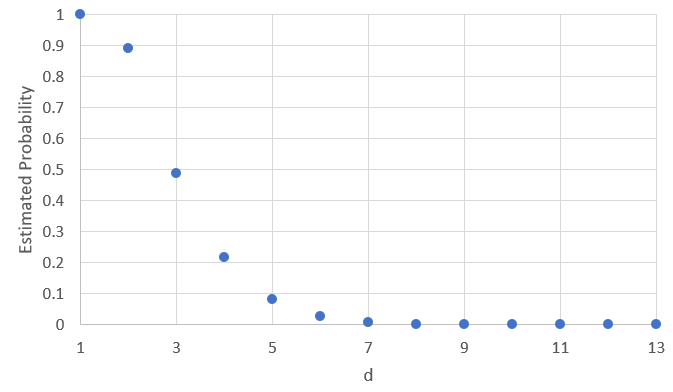
\includegraphics[width=10cm]{q1graph.png}
\caption{Graph form of results of Table 1}
\end{figure}

The function written checks divisibility of N by p by calculating $N \mod p$. For very large N we can optimise this by iterating over the digits of $N$. If $N=a_oa_1a_2\dots a_n$ we can initialise $result=0$ and iterate $result=result\times10+a_k\pmod p$ for $k=0,1\dots n$.

\subsection*{Question 2}

\begin{lemma}
If $x =\sqrt{N}$ for some positive integer $N$ then each $x_n$ may be written in the form $(r +\sqrt{N})/s$ with $r, s$ integers and $s \mid (r^
2 - N)$.
\end{lemma}

\begin{proof}

Proceed by induction. For the base case $n=0$ we have $x_0=c=x=\sqrt{N}$ so $r=0$, $s=1$ and so $s \mid (r^2 - N)$. For the inductive step, assume $x_n$ may be written as $(r +\sqrt{N})/s$ with $r,s$ integers satisfying $s \mid (r^2 - N)$. Then compute $x_{n+1}$. 

\begin{align*}
x_{n+1} &= \frac{1}{x_n-a_n}\\
		&= \frac{1}{\frac{r+\sqrt{N}}{s}-a_n}\\
		&= \frac{s}{\sqrt{N}+(r-a_ns)}\\
		&= \frac{s(\sqrt{N}-r+a_ns)}{N-r^2-a_n^2s^2+2ra_ns}\\
		&= \frac{\sqrt{N}+(a_ns-r)}{\frac{N-r^2}{s}-a_n^2s+2ra_n}\\
\end{align*}

so we have 

\begin{align*}
r' &= a_ns-r\\
s'	&= \frac{N-r^2}{s}-a_n^2s+2ra_n\\
\end{align*}

and thus 

\begin{align*}
r'^2-N &= a_n^2s^2+r^2-2a_nsr-N\\
	&= s(\frac{N-r^2}{s}-a_n^2s+2ra_n)\\
	&= ss'\\
\end{align*}

ie $s' \mid (r'^2 - N)$ as required.

\end{proof}

The expressions for $r'$ and $s'$ allow us to store $x_n$ precisely and avoid rounding errors. From IIC Number Theory, we know the sequence of partial quotients is eventually periodic, which can be identified from when $x_n$ repeats. The partial quotients for $\sqrt{N}$, N up to 50 are as follows, with the integers after the colon being repeated:

\begin{lstlisting}[breaklines]
0 ) 0 
1 ) 1 
2 ) 1 : 2
3 ) 1 : 1, 2
4 ) 2 
5 ) 2 : 4
6 ) 2 : 2, 4
7 ) 2 : 1, 1, 1, 4
8 ) 2 : 1, 4
9 ) 3 
10) 3 : 6
11) 3 : 3, 6
12) 3 : 2, 6
13) 3 : 1, 1, 1, 1, 6
14) 3 : 1, 2, 1, 6
15) 3 : 1, 6
16) 4 
17) 4 : 8
18) 4 : 4, 8
19) 4 : 2, 1, 3, 1, 2, 8
20) 4 : 2, 8
21) 4 : 1, 1, 2, 1, 1, 8
22) 4 : 1, 2, 4, 2, 1, 8
23) 4 : 1, 3, 1, 8
24) 4 : 1, 8
25) 5 
26) 5 : 10
27) 5 : 5, 10
28) 5 : 3, 2, 3, 10
29) 5 : 2, 1, 1, 2, 10
30) 5 : 2, 10
31) 5 : 1, 1, 3, 5, 3, 1, 1, 10
32) 5 : 1, 1, 1, 10
33) 5 : 1, 2, 1, 10
34) 5 : 1, 4, 1, 10
35) 5 : 1, 10
36) 6 
37) 6 : 12
38) 6 : 6, 12
39) 6 : 4, 12
40) 6 : 3, 12
41) 6 : 2, 2, 12
42) 6 : 2, 12
43) 6 : 1, 1, 3, 1, 5, 1, 3, 1, 1, 12
44) 6 : 1, 1, 1, 2, 1, 1, 1, 12
45) 6 : 1, 2, 2, 2, 1, 12
46) 6 : 1, 3, 1, 1, 2, 6, 2, 1, 1, 3, 1, 12
47) 6 : 1, 5, 1, 12
48) 6 : 1, 12
49) 7 
50) 7 : 14
\end{lstlisting}
 
We observe they all have fairly short periods, surprising since the theorem on periodicity doesn't give an indication for what the period will be. We also see that the last partial quotient before repeating is $2 \left \lfloor\sqrt{N}\right \rfloor $ TODO

\subsection*{Question 3}

The function $q3()$, using $convergents()$ produces the following data. I've included the length of the period for later reference.

\begin{lstlisting}[breaklines]
 3 [2]) -2, 1, -2, 1, -2, 1, -2, 1, -2, 1
 5 [1]) -1, 1, -1, 1, -1, 1, -1, 1, -1, 1
 7 [4]) -3, 2, -3, 1, -3, 2, -3, 1, -3, 2
12 [2]) -3, 1, -3, 1, -3, 1, -3, 1, -3, 1
31 [8]) -6, 5, -3, 2, -3, 5, -6, 1, -6, 5
\end{lstlisting}

We see the convergents always seem to contain a solution to Pells (positive) equation. Note for N a square, solving either equation gives a solution to $x^2-y^2=\pm 1$ which is clearly unsoluble. These results agree with the following theorem, proved in IIC Number Theory.

\begin{theorem}
Let n be the period of the continued fraction expansion of $\sqrt{N}$ for N not a perfect square. Then the convergent $(p_{kn-1},q_{kn-1})$ for integer k is a solution to the positive Pell equation for $kn$ even and for the negative Pell equation for $kn$ odd. In particular there are always infinitely many solutions to the positive Pell equation.
\end{theorem}



Consider the negative Pell equation $X^2-NY^2=-1$. Suppose N is divisible by 4, then mod 4 we get $X^2\equiv-1\pmod 4$ which is not soluble so there are no solutions. We can get another condition similarly. Suppose $p\mid N$ with $p\equiv 3 \pmod 4$. Then we get $X^2\equiv-1\pmod p$ but $\legendre{-1}{p}=-1$. So N cannot be divisible by 4 or be congruent to 3 mod 4.\\

Given $x,y,N$, to confirm one of Pell's equations holds, we'll use the Chinese Remainder Theorem. Take p a prime, then if $x^2-Ny^2=\pm 1$ the same must hold (mod p). By the CRT, the system

\begin{align*}
   z &= 1 \mod p_1\\
   z &= 1 \mod p_2\\
   &\vdotswithin{=} \notag \\
   z &= 1 \mod p_n\\
\end{align*}

has a unique solution mod $p_1p_2\dots p_n$. (The same holds with all 1's replaced by -1's). So to check $z=x^2-Ny^2$ is 1 it suffices the above system holds, as long as the product $p_1p_2\dots p_n$ is greater than $x^2$ and $Ny^2$. Lets use small primes, up to 113 will do, since the largest $Ny^2$ can be is $10^{45}$. \\

The reason we are using primes at all is that multiplication can be done without risk of overflow modulo. Consider multiplying x and y mod N. We write for y even, $xy = (2x)(\frac{y}{2})$ and for y odd $xy = x+ (2x)(\frac{y-1}{2})$. In the y odd case, add x mod N to the result. Now iterate the process with $x'=2x$ and $y'=\frac{y}{2}$ or $\frac{y-1}{2}$ accordingly. The process terminates when y becomes 0, which must occur as y becomes strictly smaller each iteration. In doing so we take mod N after every step and are just doing addition so worst case we store at most $2N < 2*10^{15}$. The algorithm is implemented as $modular\_multiply(x,y,mod)$\\

Our implementation of this method is $verify\_large\_pell(x,y,N)$, which is fairly fast, when tested on  x=158070671986249, y=15140424455100, n=109, and x=1766319049, y=226153980, n=61 \footnote{Obtained from \url{https://en.wikipedia.org/wiki/Pell\%27s_equation}}\\

We now wish to find some solutions to Pell's Equation. The question doesn't seem to want us to use the stated Theorem, which directly gives a valid convergent. We'll employ a trial and error approach instead, in which we calculate and then test using $verify\_large\_pell(x,y,N)$. We get the following:

\begin{lstlisting}[breaklines]

1) has no solutions (square)
2) (3,2)
3) (2,1)
4) has no solutions (square)
5) (9,4)
6) (5,2)
7) (8,3)
8) (3,1)
9) has no solutions (square)
10) (19,6)
11) (10,3)
12) (7,2)
13) (649,180)
14) (15,4)
15) (4,1)
16) has no solutions (square)
17) (33,8)
18) (17,4)
19) (170,39)
20) (9,2)
21) (55,12)
22) (197,42)
23) (24,5)
24) (5,1)
25) has no solutions (square)
26) (51,10)
27) (26,5)
28) (127,24)
29) (9801,1820)
30) (11,2)
31) (1520,273)
32) (17,3)
33) (23,4)
34) (35,6)
35) (6,1)
36) has no solutions (square)
37) (73,12)
38) (37,6)
39) (25,4)
40) (19,3)
41) (2049,320)
42) (13,2)
43) (3482,531)
44) (199,30)
45) (161,24)
46) (24335,3588)
47) (48,7)
48) (7,1)
49) has no solutions (square)
50) (99,14)
51) (50,7)
52) (649,90)
53) (66249,9100)
54) (485,66)
55) (89,12)
56) (15,2)
57) (151,20)
58) (19603,2574)
59) (530,69)
60) (31,4)
61) (1766319049,226153980)
62) (63,8)
63) (8,1)
64) has no solutions (square)
65) (129,16)
66) (65,8)
67) (48842,5967)
68) (33,4)
69) (7775,936)
70) (251,30)
71) (3480,413)
72) (17,2)
73) (2281249,267000)
74) (3699,430)
75) (26,3)
76) (57799,6630)
77) (351,40)
78) (53,6)
79) (80,9)
80) (9,1)
81) has no solutions (square)
82) (163,18)
83) (82,9)
84) (55,6)
85) (285769,30996)
86) (10405,1122)
87) (28,3)
88) (197,21)
89) (500001,53000)
90) (19,2)
91) (1574,165)
92) (1151,120)
93) (12151,1260)
94) (2143295,221064)
95) (39,4)
96) (49,5)
97) (62809633,6377352)
98) (99,10)
99) (10,1)
100) has no solutions (square)
500) (930249,41602)
501) (11242731902975,502288218432)
502) (3832352837,171046278)
503) (24648,1099)
504) (449,20)
505) (809,36)
506) (45,2)
507) (1351,60)
508) (44757606858751,1985797689600)
509) (313201220822405001,13882400040814700)
510) (271,12)
511) (4188548960,185290497)
512) (665857,29427)
513) (13771351,608020)
514) (4625,204)
515) (17406,767)
516) (16855,742)
517) (590968985399,25990786260)
518) (2367,104)
519) (14851876,651925)
520) (6499,285)
521) (32961431500035201,1444066532654320)
522) (19603,858)
523) (81810300626,3577314675)
524) (225144199,9835470)
525) (6049,264)
526) (84056091546952933775,3665019757324295532)
527) (528,23)
528) (23,1)
529) has no solutions (square)
530) (1059,46)
531) (530,23)
532) (2588599,112230)
533) (74859849,3242540)
534) (3678725,159194)
535) (1618804,69987)
536) (145925,6303)
537) (192349463,8300492)
538) (9536081203,411129654)
539) (3970,171)
540) (119071,5124)
541) (3707453360023867028800645599667005001,159395869721270110077187138775196900)
542) (4293183,184408)
543) (669337,28724)
544) (2449,105)
545) (1961,84)
546) (701,30)
547) (160177601264642,6848699678673)
548) (6083073,259856)
549) (1766319049,75384660)
550) (30580901,1303974)
\end{lstlisting}



\end{document}